\documentclass[1p]{elsarticle_modified}
%\bibliographystyle{elsarticle-num}

%\usepackage[colorlinks]{hyperref}
%\usepackage{abbrmath_seonhwa} %\Abb, \Ascr, \Acal ,\Abf, \Afrak
\usepackage{amsfonts}
\usepackage{amssymb}
\usepackage{amsmath}
\usepackage{amsthm}
\usepackage{scalefnt}
\usepackage{amsbsy}
\usepackage{kotex}
\usepackage{caption}
\usepackage{subfig}
\usepackage{color}
\usepackage{graphicx}
\usepackage{xcolor} %% white, black, red, green, blue, cyan, magenta, yellow
\usepackage{float}
\usepackage{setspace}
\usepackage{hyperref}

\usepackage{tikz}
\usetikzlibrary{arrows}

\usepackage{multirow}
\usepackage{array} % fixed length table
\usepackage{hhline}

%%%%%%%%%%%%%%%%%%%%%
\makeatletter
\renewcommand*\env@matrix[1][\arraystretch]{%
	\edef\arraystretch{#1}%
	\hskip -\arraycolsep
	\let\@ifnextchar\new@ifnextchar
	\array{*\c@MaxMatrixCols c}}
\makeatother %https://tex.stackexchange.com/questions/14071/how-can-i-increase-the-line-spacing-in-a-matrix
%%%%%%%%%%%%%%%

\usepackage[normalem]{ulem}

\newcommand{\msout}[1]{\ifmmode\text{\sout{\ensuremath{#1}}}\else\sout{#1}\fi}
%SOURCE: \msout is \stkout macro in https://tex.stackexchange.com/questions/20609/strikeout-in-math-mode

\newcommand{\cancel}[1]{
	\ifmmode
	{\color{red}\msout{#1}}
	\else
	{\color{red}\sout{#1}}
	\fi
}

\newcommand{\add}[1]{
	{\color{blue}\uwave{#1}}
}

\newcommand{\replace}[2]{
	\ifmmode
	{\color{red}\msout{#1}}{\color{blue}\uwave{#2}}
	\else
	{\color{red}\sout{#1}}{\color{blue}\uwave{#2}}
	\fi
}

\newcommand{\Sol}{\mathcal{S}} %segment
\newcommand{\D}{D} %diagram
\newcommand{\A}{\mathcal{A}} %arc


%%%%%%%%%%%%%%%%%%%%%%%%%%%%%5 test

\def\sl{\operatorname{\textup{SL}}(2,\Cbb)}
\def\psl{\operatorname{\textup{PSL}}(2,\Cbb)}
\def\quan{\mkern 1mu \triangleright \mkern 1mu}

\theoremstyle{definition}
\newtheorem{thm}{Theorem}[section]
\newtheorem{prop}[thm]{Proposition}
\newtheorem{lem}[thm]{Lemma}
\newtheorem{ques}[thm]{Question}
\newtheorem{cor}[thm]{Corollary}
\newtheorem{defn}[thm]{Definition}
\newtheorem{exam}[thm]{Example}
\newtheorem{rmk}[thm]{Remark}
\newtheorem{alg}[thm]{Algorithm}

\newcommand{\I}{\sqrt{-1}}
\begin{document}

%\begin{frontmatter}
%
%\title{Boundary parabolic representations of knots up to 8 crossings}
%
%%% Group authors per affiliation:
%\author{Yunhi Cho} 
%\address{Department of Mathematics, University of Seoul, Seoul, Korea}
%\ead{yhcho@uos.ac.kr}
%
%
%\author{Seonhwa Kim} %\fnref{s_kim}}
%\address{Center for Geometry and Physics, Institute for Basic Science, Pohang, 37673, Korea}
%\ead{ryeona17@ibs.re.kr}
%
%\author{Hyuk Kim}
%\address{Department of Mathematical Sciences, Seoul National University, Seoul 08826, Korea}
%\ead{hyukkim@snu.ac.kr}
%
%\author{Seokbeom Yoon}
%\address{Department of Mathematical Sciences, Seoul National University, Seoul, 08826,  Korea}
%\ead{sbyoon15@snu.ac.kr}
%
%\begin{abstract}
%We find all boundary parabolic representation of knots up to 8 crossings.
%
%\end{abstract}
%\begin{keyword}
%    \MSC[2010] 57M25 
%\end{keyword}
%
%\end{frontmatter}

%\linenumbers
%\tableofcontents
%
\newcommand\colored[1]{\textcolor{white}{\rule[-0.35ex]{0.8em}{1.4ex}}\kern-0.8em\color{red} #1}%
%\newcommand\colored[1]{\textcolor{white}{ #1}\kern-2.17ex	\textcolor{white}{ #1}\kern-1.81ex	\textcolor{white}{ #1}\kern-2.15ex\color{red}#1	}

{\Large $\underline{12n_{0738}~(K12n_{0738})}$}

\setlength{\tabcolsep}{10pt}
\renewcommand{\arraystretch}{1.6}
\vspace{1cm}\begin{tabular}{m{100pt}>{\centering\arraybackslash}m{274pt}}
\multirow{5}{120pt}{
	\centering
	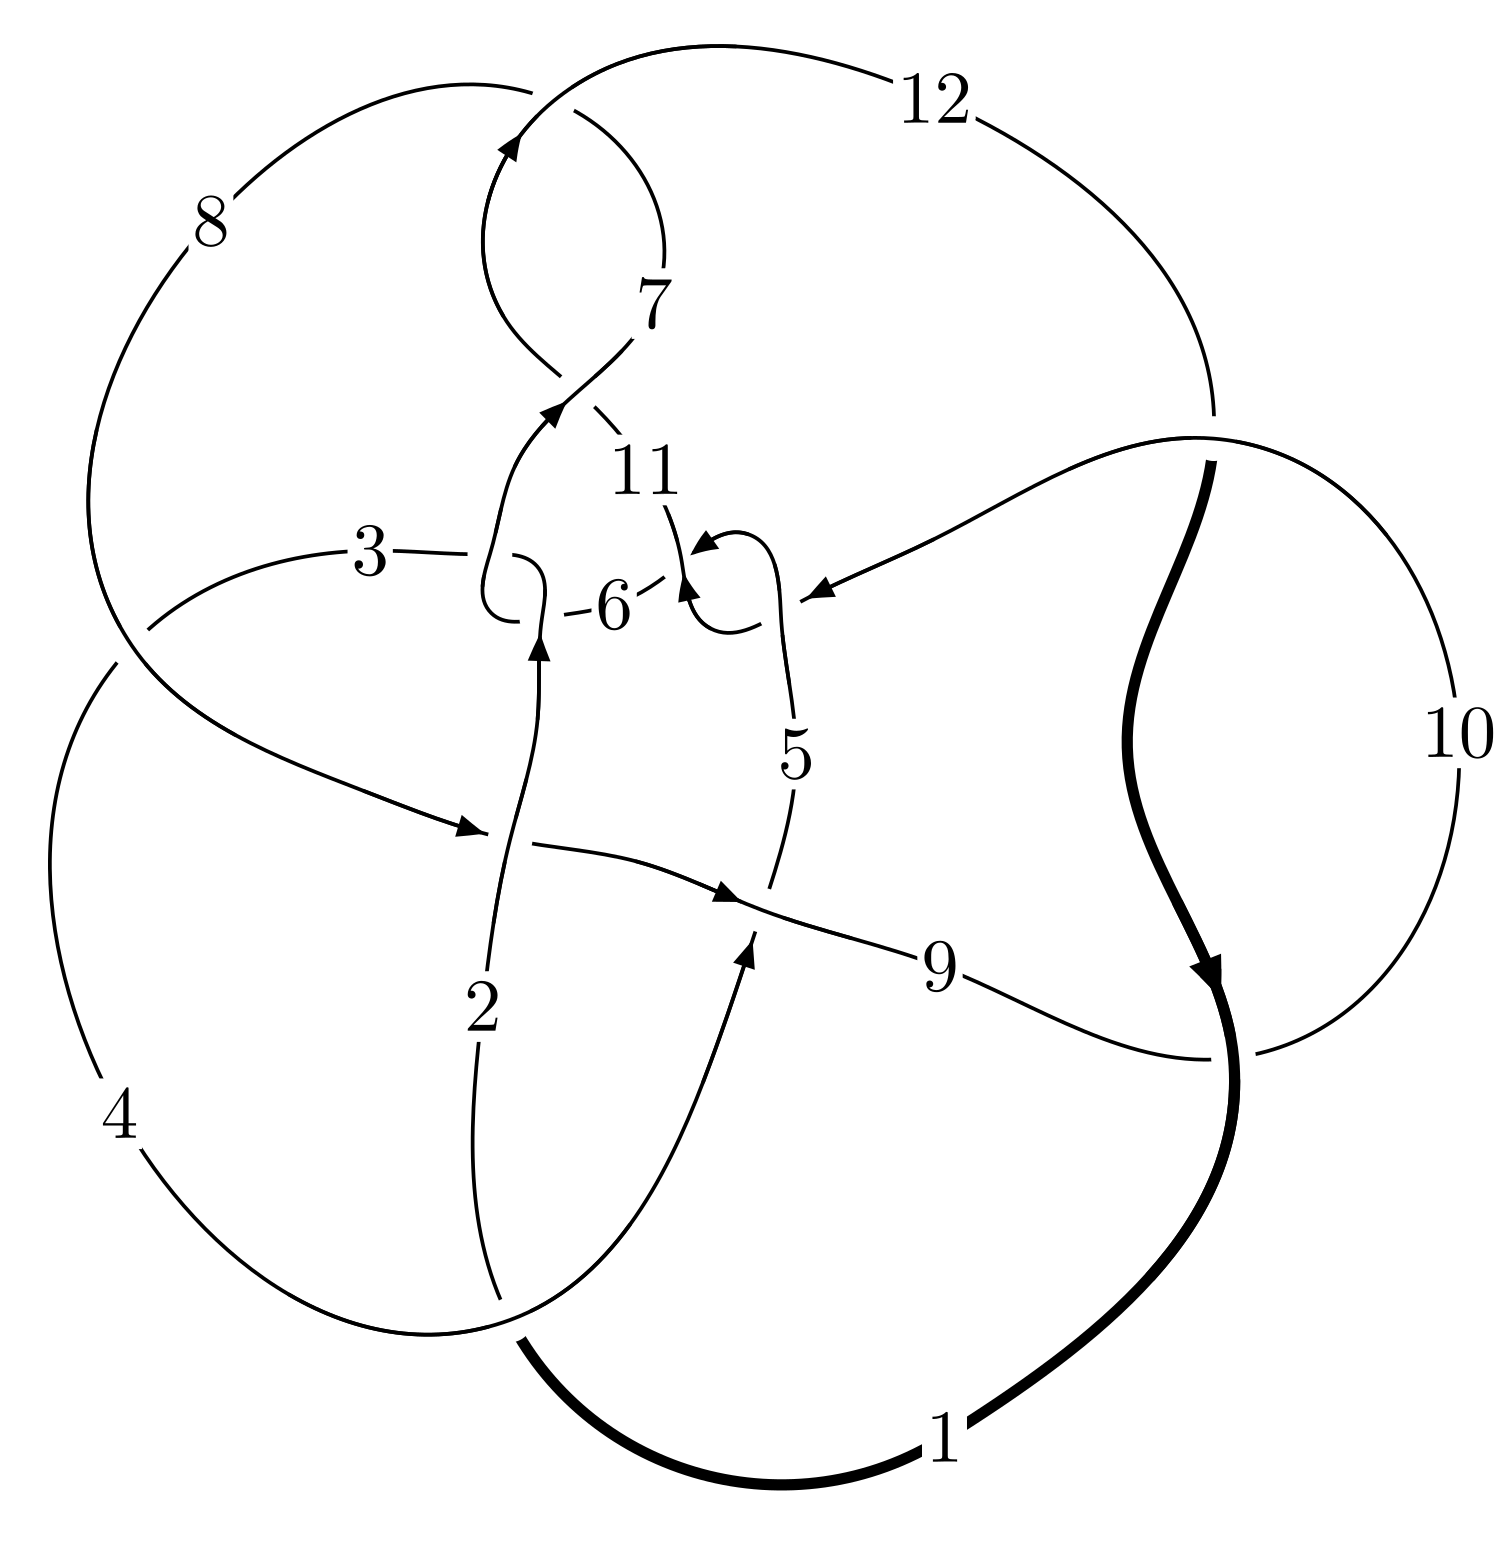
\includegraphics[width=112pt]{../../../GIT/diagram.site/Diagrams/png/2827_12n_0738.png}\\
\ \ \ A knot diagram\footnotemark}&
\allowdisplaybreaks
\textbf{Linearized knot diagam} \\
\cline{2-2}
 &
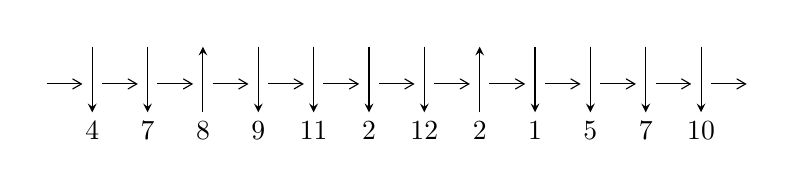
\begin{tikzpicture}[x=20pt, y=17pt]
	% nodes
	\node (C0) at (0, 0) {};
	\node (C1) at (1, 0) {};
	\node (C1U) at (1, +1) {};
	\node (C1D) at (1, -1) {4};

	\node (C2) at (2, 0) {};
	\node (C2U) at (2, +1) {};
	\node (C2D) at (2, -1) {7};

	\node (C3) at (3, 0) {};
	\node (C3U) at (3, +1) {};
	\node (C3D) at (3, -1) {8};

	\node (C4) at (4, 0) {};
	\node (C4U) at (4, +1) {};
	\node (C4D) at (4, -1) {9};

	\node (C5) at (5, 0) {};
	\node (C5U) at (5, +1) {};
	\node (C5D) at (5, -1) {11};

	\node (C6) at (6, 0) {};
	\node (C6U) at (6, +1) {};
	\node (C6D) at (6, -1) {2};

	\node (C7) at (7, 0) {};
	\node (C7U) at (7, +1) {};
	\node (C7D) at (7, -1) {12};

	\node (C8) at (8, 0) {};
	\node (C8U) at (8, +1) {};
	\node (C8D) at (8, -1) {2};

	\node (C9) at (9, 0) {};
	\node (C9U) at (9, +1) {};
	\node (C9D) at (9, -1) {1};

	\node (C10) at (10, 0) {};
	\node (C10U) at (10, +1) {};
	\node (C10D) at (10, -1) {5};

	\node (C11) at (11, 0) {};
	\node (C11U) at (11, +1) {};
	\node (C11D) at (11, -1) {7};

	\node (C12) at (12, 0) {};
	\node (C12U) at (12, +1) {};
	\node (C12D) at (12, -1) {10};
	\node (C13) at (13, 0) {};

	% arrows
	\draw[->,>={angle 60}]
	(C0) edge (C1) (C1) edge (C2) (C2) edge (C3) (C3) edge (C4) (C4) edge (C5) (C5) edge (C6) (C6) edge (C7) (C7) edge (C8) (C8) edge (C9) (C9) edge (C10) (C10) edge (C11) (C11) edge (C12) (C12) edge (C13) ;	\draw[->,>=stealth]
	(C1U) edge (C1D) (C2U) edge (C2D) (C3D) edge (C3U) (C4U) edge (C4D) (C5U) edge (C5D) (C6U) edge (C6D) (C7U) edge (C7D) (C8D) edge (C8U) (C9U) edge (C9D) (C10U) edge (C10D) (C11U) edge (C11D) (C12U) edge (C12D) ;
	\end{tikzpicture} \\
\hhline{~~} \\& 
\textbf{Solving Sequence} \\ \cline{2-2} 
 &
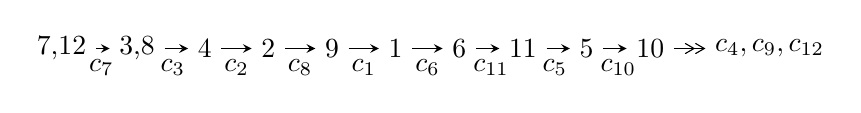
\begin{tikzpicture}[x=23pt, y=7pt]
	% node
	\node (A0) at (-1/8, 0) {7,12};
	\node (A1) at (17/16, 0) {3,8};
	\node (A2) at (17/8, 0) {4};
	\node (A3) at (25/8, 0) {2};
	\node (A4) at (33/8, 0) {9};
	\node (A5) at (41/8, 0) {1};
	\node (A6) at (49/8, 0) {6};
	\node (A7) at (57/8, 0) {11};
	\node (A8) at (65/8, 0) {5};
	\node (A9) at (73/8, 0) {10};
	\node (C1) at (1/2, -1) {$c_{7}$};
	\node (C2) at (13/8, -1) {$c_{3}$};
	\node (C3) at (21/8, -1) {$c_{2}$};
	\node (C4) at (29/8, -1) {$c_{8}$};
	\node (C5) at (37/8, -1) {$c_{1}$};
	\node (C6) at (45/8, -1) {$c_{6}$};
	\node (C7) at (53/8, -1) {$c_{11}$};
	\node (C8) at (61/8, -1) {$c_{5}$};
	\node (C9) at (69/8, -1) {$c_{10}$};
	\node (A10) at (11, 0) {$c_{4},c_{9},c_{12}$};

	% edge
	\draw[->,>=stealth]	
	(A0) edge (A1) (A1) edge (A2) (A2) edge (A3) (A3) edge (A4) (A4) edge (A5) (A5) edge (A6) (A6) edge (A7) (A7) edge (A8) (A8) edge (A9) ;
	\draw[->>,>={angle 60}]	
	(A9) edge (A10);
\end{tikzpicture} \\ 

\end{tabular} \\

\footnotetext{
The image of knot diagram is generated by the software ``\textbf{Draw programme}" developed by Andrew Bartholomew(\url{http://www.layer8.co.uk/maths/draw/index.htm\#Running-draw}), where we modified some parts for our purpose(\url{https://github.com/CATsTAILs/LinksPainter}).
}\phantom \\ \newline 
\centering \textbf{Ideals for irreducible components\footnotemark of $X_{\text{par}}$} 
 
\begin{align*}
I^u_{1}&=\langle 
-9.79475\times10^{256} u^{88}+1.43387\times10^{257} u^{87}+\cdots+1.05146\times10^{255} b+1.97384\times10^{257},\\
\phantom{I^u_{1}}&\phantom{= \langle  }1.78518\times10^{256} u^{88}-1.84553\times10^{256} u^{87}+\cdots+5.25732\times10^{254} a+5.76703\times10^{255},\;u^{89}-2 u^{88}+\cdots-14 u+1\rangle \\
I^u_{2}&=\langle 
-2542623226711 u^{21}-5879535861531 u^{20}+\cdots+4155085006409 b-2615410115873,\\
\phantom{I^u_{2}}&\phantom{= \langle  }6655009669836 u^{21}+10389904986854 u^{20}+\cdots+4155085006409 a+4757958548853,\\
\phantom{I^u_{2}}&\phantom{= \langle  }u^{22}+2 u^{21}+\cdots+u+1\rangle \\
I^u_{3}&=\langle 
b+1,\;a^3+a^2+1,\;u-1\rangle \\
\\
\end{align*}
\raggedright * 3 irreducible components of $\dim_{\mathbb{C}}=0$, with total 114 representations.\\
\footnotetext{All coefficients of polynomials are rational numbers. But the coefficients are sometimes approximated in decimal forms when there is not enough margin.}
\newpage
\renewcommand{\arraystretch}{1}
\centering \section*{I. $I^u_{1}= \langle -9.79\times10^{256} u^{88}+1.43\times10^{257} u^{87}+\cdots+1.05\times10^{255} b+1.97\times10^{257},\;1.79\times10^{256} u^{88}-1.85\times10^{256} u^{87}+\cdots+5.26\times10^{254} a+5.77\times10^{255},\;u^{89}-2 u^{88}+\cdots-14 u+1 \rangle$}
\flushleft \textbf{(i) Arc colorings}\\
\begin{tabular}{m{7pt} m{180pt} m{7pt} m{180pt} }
\flushright $a_{7}=$&$\begin{pmatrix}1\\0\end{pmatrix}$ \\
\flushright $a_{12}=$&$\begin{pmatrix}0\\u\end{pmatrix}$ \\
\flushright $a_{3}=$&$\begin{pmatrix}-33.9561 u^{88}+35.1040 u^{87}+\cdots-18.7014 u-10.9695\\93.1534 u^{88}-136.369 u^{87}+\cdots+2197.99 u-187.723\end{pmatrix}$ \\
\flushright $a_{8}=$&$\begin{pmatrix}1\\u^2\end{pmatrix}$ \\
\flushright $a_{4}=$&$\begin{pmatrix}81.4663 u^{88}-132.400 u^{87}+\cdots+2604.65 u-231.500\\128.707 u^{88}-187.467 u^{87}+\cdots+2969.35 u-251.064\end{pmatrix}$ \\
\flushright $a_{2}=$&$\begin{pmatrix}59.1974 u^{88}-101.265 u^{87}+\cdots+2179.29 u-198.692\\93.1534 u^{88}-136.369 u^{87}+\cdots+2197.99 u-187.723\end{pmatrix}$ \\
\flushright $a_{9}=$&$\begin{pmatrix}75.1897 u^{88}-109.168 u^{87}+\cdots+1597.75 u-115.139\\-3.66417 u^{88}+10.3005 u^{87}+\cdots-159.896 u+11.8154\end{pmatrix}$ \\
\flushright $a_{1}=$&$\begin{pmatrix}16.7378 u^{88}-44.3957 u^{87}+\cdots+1381.92 u-131.287\\-16.2704 u^{88}+14.4942 u^{87}+\cdots+69.9257 u-18.6626\end{pmatrix}$ \\
\flushright $a_{6}=$&$\begin{pmatrix}62.4914 u^{88}-86.8598 u^{87}+\cdots+1097.29 u-65.6761\\18.6435 u^{88}-21.1867 u^{87}+\cdots+311.334 u-26.3076\end{pmatrix}$ \\
\flushright $a_{11}=$&$\begin{pmatrix}u\\u\end{pmatrix}$ \\
\flushright $a_{5}=$&$\begin{pmatrix}53.5827 u^{88}-71.8606 u^{87}+\cdots+832.817 u-43.6534\\9.73484 u^{88}-6.18748 u^{87}+\cdots+46.8642 u-4.28488\end{pmatrix}$ \\
\flushright $a_{10}=$&$\begin{pmatrix}-50.5975 u^{88}+85.3027 u^{87}+\cdots-1981.82 u+202.076\\63.8761 u^{88}-100.827 u^{87}+\cdots+1699.64 u-142.543\end{pmatrix}$\\&\end{tabular}
\flushleft \textbf{(ii) Obstruction class $= -1$}\\~\\
\flushleft \textbf{(iii) Cusp Shapes $= 99.2749 u^{88}-167.730 u^{87}+\cdots+2872.55 u-234.918$}\\~\\
\newpage\renewcommand{\arraystretch}{1}
\flushleft \textbf{(iv) u-Polynomials at the component}\newline \\
\begin{tabular}{m{50pt}|m{274pt}}
Crossings & \hspace{64pt}u-Polynomials at each crossing \\
\hline $$\begin{aligned}c_{1}\end{aligned}$$&$\begin{aligned}
&u^{89}-2 u^{88}+\cdots+3224 u-173
\end{aligned}$\\
\hline $$\begin{aligned}c_{2},c_{6}\end{aligned}$$&$\begin{aligned}
&u^{89}+3 u^{88}+\cdots+2143 u+220
\end{aligned}$\\
\hline $$\begin{aligned}c_{3}\end{aligned}$$&$\begin{aligned}
&u^{89}+2 u^{88}+\cdots+42280112 u+2904067
\end{aligned}$\\
\hline $$\begin{aligned}c_{4}\end{aligned}$$&$\begin{aligned}
&u^{89}+u^{88}+\cdots+76 u^2+16
\end{aligned}$\\
\hline $$\begin{aligned}c_{5},c_{10}\end{aligned}$$&$\begin{aligned}
&u^{89}+u^{88}+\cdots-1398 u+457
\end{aligned}$\\
\hline $$\begin{aligned}c_{7},c_{11}\end{aligned}$$&$\begin{aligned}
&u^{89}-2 u^{88}+\cdots-14 u+1
\end{aligned}$\\
\hline $$\begin{aligned}c_{8}\end{aligned}$$&$\begin{aligned}
&u^{89}+3 u^{88}+\cdots+37920 u+3361
\end{aligned}$\\
\hline $$\begin{aligned}c_{9},c_{12}\end{aligned}$$&$\begin{aligned}
&u^{89}+u^{88}+\cdots+349 u+211
\end{aligned}$\\
\hline
\end{tabular}\\~\\
\newpage\renewcommand{\arraystretch}{1}
\flushleft \textbf{(v) Riley Polynomials at the component}\newline \\
\begin{tabular}{m{50pt}|m{274pt}}
Crossings & \hspace{64pt}Riley Polynomials at each crossing \\
\hline $$\begin{aligned}c_{1}\end{aligned}$$&$\begin{aligned}
&y^{89}+26 y^{88}+\cdots+2490152 y-29929
\end{aligned}$\\
\hline $$\begin{aligned}c_{2},c_{6}\end{aligned}$$&$\begin{aligned}
&y^{89}+63 y^{88}+\cdots-2481871 y-48400
\end{aligned}$\\
\hline $$\begin{aligned}c_{3}\end{aligned}$$&$\begin{aligned}
&y^{89}-56 y^{88}+\cdots-83395183689034 y-8433605140489
\end{aligned}$\\
\hline $$\begin{aligned}c_{4}\end{aligned}$$&$\begin{aligned}
&y^{89}+3 y^{88}+\cdots-2432 y-256
\end{aligned}$\\
\hline $$\begin{aligned}c_{5},c_{10}\end{aligned}$$&$\begin{aligned}
&y^{89}-43 y^{88}+\cdots+3827190 y-208849
\end{aligned}$\\
\hline $$\begin{aligned}c_{7},c_{11}\end{aligned}$$&$\begin{aligned}
&y^{89}-24 y^{88}+\cdots+66 y-1
\end{aligned}$\\
\hline $$\begin{aligned}c_{8}\end{aligned}$$&$\begin{aligned}
&y^{89}-9 y^{88}+\cdots+460345940 y-11296321
\end{aligned}$\\
\hline $$\begin{aligned}c_{9},c_{12}\end{aligned}$$&$\begin{aligned}
&y^{89}+55 y^{88}+\cdots-1038699 y-44521
\end{aligned}$\\
\hline
\end{tabular}\\~\\
\newpage\flushleft \textbf{(vi) Complex Volumes and Cusp Shapes}
$$\begin{array}{c|c|c}  
\text{Solutions to }I^u_{1}& \I (\text{vol} + \sqrt{-1}CS) & \text{Cusp shape}\\
 \hline 
\begin{aligned}
u &= \phantom{-}0.728707 + 0.689660 I \\
a &= \phantom{-}1.140920 - 0.798950 I \\
b &= -0.106997 + 1.343020 I\end{aligned}
 & \phantom{-}3.36537 + 3.15246 I & \phantom{-0.000000 } 0 \\ \hline\begin{aligned}
u &= \phantom{-}0.728707 - 0.689660 I \\
a &= \phantom{-}1.140920 + 0.798950 I \\
b &= -0.106997 - 1.343020 I\end{aligned}
 & \phantom{-}3.36537 - 3.15246 I & \phantom{-0.000000 } 0 \\ \hline\begin{aligned}
u &= -0.924993 + 0.174397 I \\
a &= \phantom{-}1.57826 + 0.33149 I \\
b &= \phantom{-}0.991171 - 0.061075 I\end{aligned}
 & -3.52619 - 0.12569 I & \phantom{-0.000000 } 0 \\ \hline\begin{aligned}
u &= -0.924993 - 0.174397 I \\
a &= \phantom{-}1.57826 - 0.33149 I \\
b &= \phantom{-}0.991171 + 0.061075 I\end{aligned}
 & -3.52619 + 0.12569 I & \phantom{-0.000000 } 0 \\ \hline\begin{aligned}
u &= \phantom{-}1.116820 + 0.152077 I \\
a &= \phantom{-}0.650111 + 0.740802 I \\
b &= -0.759825 + 0.290326 I\end{aligned}
 & -3.17613 + 0.89707 I & \phantom{-0.000000 } 0 \\ \hline\begin{aligned}
u &= \phantom{-}1.116820 - 0.152077 I \\
a &= \phantom{-}0.650111 - 0.740802 I \\
b &= -0.759825 - 0.290326 I\end{aligned}
 & -3.17613 - 0.89707 I & \phantom{-0.000000 } 0 \\ \hline\begin{aligned}
u &= \phantom{-}0.450061 + 0.744605 I \\
a &= \phantom{-}0.607261 - 0.124059 I \\
b &= \phantom{-}0.502872 + 0.181456 I\end{aligned}
 & \phantom{-}3.61994 - 0.64342 I & \phantom{-0.000000 } 0 \\ \hline\begin{aligned}
u &= \phantom{-}0.450061 - 0.744605 I \\
a &= \phantom{-}0.607261 + 0.124059 I \\
b &= \phantom{-}0.502872 - 0.181456 I\end{aligned}
 & \phantom{-}3.61994 + 0.64342 I & \phantom{-0.000000 } 0 \\ \hline\begin{aligned}
u &= -0.865942 + 0.013321 I \\
a &= -0.377046 + 1.305970 I \\
b &= \phantom{-}0.12951 - 1.45777 I\end{aligned}
 & -0.82448 - 6.19029 I & \phantom{-0.000000 } 0 \\ \hline\begin{aligned}
u &= -0.865942 - 0.013321 I \\
a &= -0.377046 - 1.305970 I \\
b &= \phantom{-}0.12951 + 1.45777 I\end{aligned}
 & -0.82448 + 6.19029 I & \phantom{-0.000000 } 0\\
 \hline 
 \end{array}$$\newpage$$\begin{array}{c|c|c}  
\text{Solutions to }I^u_{1}& \I (\text{vol} + \sqrt{-1}CS) & \text{Cusp shape}\\
 \hline 
\begin{aligned}
u &= -0.573452 + 0.587260 I \\
a &= -0.60537 - 1.48602 I \\
b &= -1.077630 + 0.711416 I\end{aligned}
 & -0.31660 + 4.57592 I & \phantom{-0.000000 } 0 \\ \hline\begin{aligned}
u &= -0.573452 - 0.587260 I \\
a &= -0.60537 + 1.48602 I \\
b &= -1.077630 - 0.711416 I\end{aligned}
 & -0.31660 - 4.57592 I & \phantom{-0.000000 } 0 \\ \hline\begin{aligned}
u &= -0.809930 + 0.027084 I \\
a &= \phantom{-}0.238299 - 0.326731 I \\
b &= -1.188020 - 0.459108 I\end{aligned}
 & -1.67659 - 1.76730 I & \phantom{-0.000000 } 0 \\ \hline\begin{aligned}
u &= -0.809930 - 0.027084 I \\
a &= \phantom{-}0.238299 + 0.326731 I \\
b &= -1.188020 + 0.459108 I\end{aligned}
 & -1.67659 + 1.76730 I & \phantom{-0.000000 } 0 \\ \hline\begin{aligned}
u &= -1.186060 + 0.122031 I \\
a &= \phantom{-}0.473953 - 0.313586 I \\
b &= -0.677351 - 0.634263 I\end{aligned}
 & -2.10870 - 1.82799 I & \phantom{-0.000000 } 0 \\ \hline\begin{aligned}
u &= -1.186060 - 0.122031 I \\
a &= \phantom{-}0.473953 + 0.313586 I \\
b &= -0.677351 + 0.634263 I\end{aligned}
 & -2.10870 + 1.82799 I & \phantom{-0.000000 } 0 \\ \hline\begin{aligned}
u &= -0.878350 + 0.815051 I \\
a &= -0.500476 - 1.315300 I \\
b &= -0.76164 + 1.34733 I\end{aligned}
 & \phantom{-}0.99618 + 5.42464 I & \phantom{-0.000000 } 0 \\ \hline\begin{aligned}
u &= -0.878350 - 0.815051 I \\
a &= -0.500476 + 1.315300 I \\
b &= -0.76164 - 1.34733 I\end{aligned}
 & \phantom{-}0.99618 - 5.42464 I & \phantom{-0.000000 } 0 \\ \hline\begin{aligned}
u &= \phantom{-}0.726246 + 0.975893 I \\
a &= \phantom{-}0.640522 - 0.768375 I \\
b &= \phantom{-}0.351698 + 1.075030 I\end{aligned}
 & \phantom{-}4.14888 - 0.87827 I & \phantom{-0.000000 } 0 \\ \hline\begin{aligned}
u &= \phantom{-}0.726246 - 0.975893 I \\
a &= \phantom{-}0.640522 + 0.768375 I \\
b &= \phantom{-}0.351698 - 1.075030 I\end{aligned}
 & \phantom{-}4.14888 + 0.87827 I & \phantom{-0.000000 } 0\\
 \hline 
 \end{array}$$\newpage$$\begin{array}{c|c|c}  
\text{Solutions to }I^u_{1}& \I (\text{vol} + \sqrt{-1}CS) & \text{Cusp shape}\\
 \hline 
\begin{aligned}
u &= -0.985705 + 0.750992 I \\
a &= \phantom{-}0.782971 + 0.642116 I \\
b &= -0.109357 - 1.160930 I\end{aligned}
 & \phantom{-}0.662776 + 0.539516 I & \phantom{-0.000000 } 0 \\ \hline\begin{aligned}
u &= -0.985705 - 0.750992 I \\
a &= \phantom{-}0.782971 - 0.642116 I \\
b &= -0.109357 + 1.160930 I\end{aligned}
 & \phantom{-}0.662776 - 0.539516 I & \phantom{-0.000000 } 0 \\ \hline\begin{aligned}
u &= -0.712728 + 1.015920 I \\
a &= \phantom{-}0.499103 + 1.235100 I \\
b &= \phantom{-}0.29416 - 1.61372 I\end{aligned}
 & \phantom{-}9.54462 - 2.29743 I & \phantom{-0.000000 } 0 \\ \hline\begin{aligned}
u &= -0.712728 - 1.015920 I \\
a &= \phantom{-}0.499103 - 1.235100 I \\
b &= \phantom{-}0.29416 + 1.61372 I\end{aligned}
 & \phantom{-}9.54462 + 2.29743 I & \phantom{-0.000000 } 0 \\ \hline\begin{aligned}
u &= \phantom{-}0.766930 + 0.993698 I \\
a &= \phantom{-}0.401340 - 0.947871 I \\
b &= \phantom{-}0.54402 + 1.44826 I\end{aligned}
 & \phantom{-}4.50282 - 1.08927 I & \phantom{-0.000000 } 0 \\ \hline\begin{aligned}
u &= \phantom{-}0.766930 - 0.993698 I \\
a &= \phantom{-}0.401340 + 0.947871 I \\
b &= \phantom{-}0.54402 - 1.44826 I\end{aligned}
 & \phantom{-}4.50282 + 1.08927 I & \phantom{-0.000000 } 0 \\ \hline\begin{aligned}
u &= \phantom{-}1.013200 + 0.753764 I \\
a &= -0.646652 + 1.230910 I \\
b &= -0.70501 - 1.64006 I\end{aligned}
 & \phantom{-}2.56199 - 8.83087 I & \phantom{-0.000000 } 0 \\ \hline\begin{aligned}
u &= \phantom{-}1.013200 - 0.753764 I \\
a &= -0.646652 - 1.230910 I \\
b &= -0.70501 + 1.64006 I\end{aligned}
 & \phantom{-}2.56199 + 8.83087 I & \phantom{-0.000000 } 0 \\ \hline\begin{aligned}
u &= -0.732612 + 1.030540 I \\
a &= \phantom{-}0.156776 + 1.052220 I \\
b &= \phantom{-}0.57412 - 1.73131 I\end{aligned}
 & \phantom{-}6.53176 + 7.27006 I & \phantom{-0.000000 } 0 \\ \hline\begin{aligned}
u &= -0.732612 - 1.030540 I \\
a &= \phantom{-}0.156776 - 1.052220 I \\
b &= \phantom{-}0.57412 + 1.73131 I\end{aligned}
 & \phantom{-}6.53176 - 7.27006 I & \phantom{-0.000000 } 0\\
 \hline 
 \end{array}$$\newpage$$\begin{array}{c|c|c}  
\text{Solutions to }I^u_{1}& \I (\text{vol} + \sqrt{-1}CS) & \text{Cusp shape}\\
 \hline 
\begin{aligned}
u &= -0.607390 + 0.408610 I \\
a &= \phantom{-}0.66595 - 1.34345 I \\
b &= -0.190565 + 0.778107 I\end{aligned}
 & -1.32281 + 1.49993 I & -8.00000 + 0. I\phantom{ +0.000000I} \\ \hline\begin{aligned}
u &= -0.607390 - 0.408610 I \\
a &= \phantom{-}0.66595 + 1.34345 I \\
b &= -0.190565 - 0.778107 I\end{aligned}
 & -1.32281 - 1.49993 I & -8.00000 + 0. I\phantom{ +0.000000I} \\ \hline\begin{aligned}
u &= \phantom{-}0.581342 + 0.441443 I \\
a &= -0.212475 - 0.031319 I \\
b &= \phantom{-}1.93552 - 0.28067 I\end{aligned}
 & \phantom{-}0.71957 - 8.87941 I & -8.0000 + 13.4036 I \\ \hline\begin{aligned}
u &= \phantom{-}0.581342 - 0.441443 I \\
a &= -0.212475 + 0.031319 I \\
b &= \phantom{-}1.93552 + 0.28067 I\end{aligned}
 & \phantom{-}0.71957 + 8.87941 I & -8.0000 - 13.4036 I \\ \hline\begin{aligned}
u &= \phantom{-}0.720659 + 0.071260 I \\
a &= \phantom{-}2.08430 - 0.32839 I \\
b &= \phantom{-}1.001690 - 0.367941 I\end{aligned}
 & -0.05018 + 6.72143 I & -13.2759 - 5.0382 I \\ \hline\begin{aligned}
u &= \phantom{-}0.720659 - 0.071260 I \\
a &= \phantom{-}2.08430 + 0.32839 I \\
b &= \phantom{-}1.001690 + 0.367941 I\end{aligned}
 & -0.05018 - 6.72143 I & -13.2759 + 5.0382 I \\ \hline\begin{aligned}
u &= -0.476229 + 0.525739 I \\
a &= -0.142712 - 0.221460 I \\
b &= \phantom{-}1.48007 + 0.83547 I\end{aligned}
 & -1.81194 + 3.10417 I & -8.00000 - 9.84544 I \\ \hline\begin{aligned}
u &= -0.476229 - 0.525739 I \\
a &= -0.142712 + 0.221460 I \\
b &= \phantom{-}1.48007 - 0.83547 I\end{aligned}
 & -1.81194 - 3.10417 I & -8.00000 + 9.84544 I \\ \hline\begin{aligned}
u &= \phantom{-}0.688408 + 0.125680 I \\
a &= -0.276936 + 0.559711 I \\
b &= -1.53936 + 0.11618 I\end{aligned}
 & -2.46249 - 0.67631 I & -8.00000 + 10.85950 I \\ \hline\begin{aligned}
u &= \phantom{-}0.688408 - 0.125680 I \\
a &= -0.276936 - 0.559711 I \\
b &= -1.53936 - 0.11618 I\end{aligned}
 & -2.46249 + 0.67631 I & -8.00000 - 10.85950 I\\
 \hline 
 \end{array}$$\newpage$$\begin{array}{c|c|c}  
\text{Solutions to }I^u_{1}& \I (\text{vol} + \sqrt{-1}CS) & \text{Cusp shape}\\
 \hline 
\begin{aligned}
u &= -0.644054 + 0.260652 I \\
a &= \phantom{-}1.14759 - 1.42214 I \\
b &= -0.247479 + 0.278785 I\end{aligned}
 & -1.54586 + 1.12108 I & -11.00706 - 6.04709 I \\ \hline\begin{aligned}
u &= -0.644054 - 0.260652 I \\
a &= \phantom{-}1.14759 + 1.42214 I \\
b &= -0.247479 - 0.278785 I\end{aligned}
 & -1.54586 - 1.12108 I & -11.00706 + 6.04709 I \\ \hline\begin{aligned}
u &= \phantom{-}0.620239 + 0.221199 I \\
a &= -1.06970 - 2.54323 I \\
b &= -0.075257 - 0.139231 I\end{aligned}
 & -3.44636 - 3.28123 I & -20.2992 + 8.3870 I \\ \hline\begin{aligned}
u &= \phantom{-}0.620239 - 0.221199 I \\
a &= -1.06970 + 2.54323 I \\
b &= -0.075257 + 0.139231 I\end{aligned}
 & -3.44636 + 3.28123 I & -20.2992 - 8.3870 I \\ \hline\begin{aligned}
u &= -0.445574 + 0.477651 I \\
a &= -2.96309 + 1.38824 I \\
b &= \phantom{-}0.116212 + 0.104340 I\end{aligned}
 & \phantom{-}1.10496 + 8.28971 I & -4.3178 - 14.5248 I \\ \hline\begin{aligned}
u &= -0.445574 - 0.477651 I \\
a &= -2.96309 - 1.38824 I \\
b &= \phantom{-}0.116212 - 0.104340 I\end{aligned}
 & \phantom{-}1.10496 - 8.28971 I & -4.3178 + 14.5248 I \\ \hline\begin{aligned}
u &= \phantom{-}0.855189 + 1.043680 I \\
a &= -0.407496 + 0.805868 I \\
b &= \phantom{-}0.24636 - 1.41483 I\end{aligned}
 & \phantom{-}7.31163 - 1.88418 I & \phantom{-0.000000 } 0 \\ \hline\begin{aligned}
u &= \phantom{-}0.855189 - 1.043680 I \\
a &= -0.407496 - 0.805868 I \\
b &= \phantom{-}0.24636 + 1.41483 I\end{aligned}
 & \phantom{-}7.31163 + 1.88418 I & \phantom{-0.000000 } 0 \\ \hline\begin{aligned}
u &= \phantom{-}0.429882 + 0.485314 I \\
a &= \phantom{-}0.85439 + 2.04202 I \\
b &= -0.483871 - 1.087000 I\end{aligned}
 & -0.54805 - 3.51803 I & -5.26955 + 4.96976 I \\ \hline\begin{aligned}
u &= \phantom{-}0.429882 - 0.485314 I \\
a &= \phantom{-}0.85439 - 2.04202 I \\
b &= -0.483871 + 1.087000 I\end{aligned}
 & -0.54805 + 3.51803 I & -5.26955 - 4.96976 I\\
 \hline 
 \end{array}$$\newpage$$\begin{array}{c|c|c}  
\text{Solutions to }I^u_{1}& \I (\text{vol} + \sqrt{-1}CS) & \text{Cusp shape}\\
 \hline 
\begin{aligned}
u &= -0.780322 + 1.124850 I \\
a &= \phantom{-}0.879309 + 0.837722 I \\
b &= \phantom{-}0.042420 - 1.053150 I\end{aligned}
 & \phantom{-}5.37297 + 0.17301 I & \phantom{-0.000000 } 0 \\ \hline\begin{aligned}
u &= -0.780322 - 1.124850 I \\
a &= \phantom{-}0.879309 - 0.837722 I \\
b &= \phantom{-}0.042420 + 1.053150 I\end{aligned}
 & \phantom{-}5.37297 - 0.17301 I & \phantom{-0.000000 } 0 \\ \hline\begin{aligned}
u &= -0.810003 + 1.147870 I \\
a &= -0.579327 - 0.691089 I \\
b &= \phantom{-}0.19153 + 1.41504 I\end{aligned}
 & \phantom{-}2.04685 - 4.05320 I & \phantom{-0.000000 } 0 \\ \hline\begin{aligned}
u &= -0.810003 - 1.147870 I \\
a &= -0.579327 + 0.691089 I \\
b &= \phantom{-}0.19153 - 1.41504 I\end{aligned}
 & \phantom{-}2.04685 + 4.05320 I & \phantom{-0.000000 } 0 \\ \hline\begin{aligned}
u &= \phantom{-}1.122200 + 0.854316 I \\
a &= -0.583374 + 0.657925 I \\
b &= -0.33959 - 1.41890 I\end{aligned}
 & \phantom{-}3.37656 - 5.71824 I & \phantom{-0.000000 } 0 \\ \hline\begin{aligned}
u &= \phantom{-}1.122200 - 0.854316 I \\
a &= -0.583374 - 0.657925 I \\
b &= -0.33959 + 1.41890 I\end{aligned}
 & \phantom{-}3.37656 + 5.71824 I & \phantom{-0.000000 } 0 \\ \hline\begin{aligned}
u &= -1.150330 + 0.818490 I \\
a &= -0.863157 - 0.795066 I \\
b &= -0.22259 + 1.57983 I\end{aligned}
 & \phantom{-}8.14222 + 9.05246 I & \phantom{-0.000000 } 0 \\ \hline\begin{aligned}
u &= -1.150330 - 0.818490 I \\
a &= -0.863157 + 0.795066 I \\
b &= -0.22259 - 1.57983 I\end{aligned}
 & \phantom{-}8.14222 - 9.05246 I & \phantom{-0.000000 } 0 \\ \hline\begin{aligned}
u &= \phantom{-}1.12526 + 0.86285 I \\
a &= -0.357076 + 0.892757 I \\
b &= -0.47716 - 1.43875 I\end{aligned}
 & \phantom{-}2.91341 - 5.91259 I & \phantom{-0.000000 } 0 \\ \hline\begin{aligned}
u &= \phantom{-}1.12526 - 0.86285 I \\
a &= -0.357076 - 0.892757 I \\
b &= -0.47716 + 1.43875 I\end{aligned}
 & \phantom{-}2.91341 + 5.91259 I & \phantom{-0.000000 } 0\\
 \hline 
 \end{array}$$\newpage$$\begin{array}{c|c|c}  
\text{Solutions to }I^u_{1}& \I (\text{vol} + \sqrt{-1}CS) & \text{Cusp shape}\\
 \hline 
\begin{aligned}
u &= \phantom{-}1.08481 + 0.92394 I \\
a &= \phantom{-}0.665171 - 0.977161 I \\
b &= \phantom{-}0.73889 + 1.21253 I\end{aligned}
 & \phantom{-}6.57099 - 5.29222 I & \phantom{-0.000000 } 0 \\ \hline\begin{aligned}
u &= \phantom{-}1.08481 - 0.92394 I \\
a &= \phantom{-}0.665171 + 0.977161 I \\
b &= \phantom{-}0.73889 - 1.21253 I\end{aligned}
 & \phantom{-}6.57099 + 5.29222 I & \phantom{-0.000000 } 0 \\ \hline\begin{aligned}
u &= \phantom{-}0.76985 + 1.20914 I \\
a &= -0.249525 + 1.327490 I \\
b &= -0.388594 - 1.129600 I\end{aligned}
 & \phantom{-}6.48905 - 4.72393 I & \phantom{-0.000000 } 0 \\ \hline\begin{aligned}
u &= \phantom{-}0.76985 - 1.20914 I \\
a &= -0.249525 - 1.327490 I \\
b &= -0.388594 + 1.129600 I\end{aligned}
 & \phantom{-}6.48905 + 4.72393 I & \phantom{-0.000000 } 0 \\ \hline\begin{aligned}
u &= \phantom{-}0.81489 + 1.19005 I \\
a &= -0.679307 + 0.759719 I \\
b &= \phantom{-}0.229063 - 1.393780 I\end{aligned}
 & \phantom{-}6.15465 + 10.11680 I & \phantom{-0.000000 } 0 \\ \hline\begin{aligned}
u &= \phantom{-}0.81489 - 1.19005 I \\
a &= -0.679307 - 0.759719 I \\
b &= \phantom{-}0.229063 + 1.393780 I\end{aligned}
 & \phantom{-}6.15465 - 10.11680 I & \phantom{-0.000000 } 0 \\ \hline\begin{aligned}
u &= \phantom{-}0.548991 + 0.053107 I \\
a &= -0.61886 - 1.53164 I \\
b &= -0.19159 + 1.61911 I\end{aligned}
 & -3.16683 + 2.11548 I & -19.9398 + 0.6159 I \\ \hline\begin{aligned}
u &= \phantom{-}0.548991 - 0.053107 I \\
a &= -0.61886 + 1.53164 I \\
b &= -0.19159 - 1.61911 I\end{aligned}
 & -3.16683 - 2.11548 I & -19.9398 - 0.6159 I \\ \hline\begin{aligned}
u &= \phantom{-}0.320160 + 0.435342 I \\
a &= -0.30304 - 1.39831 I \\
b &= -0.168673 - 0.492183 I\end{aligned}
 & \phantom{-}2.82976 - 3.05132 I & -6.01961 + 4.35621 I \\ \hline\begin{aligned}
u &= \phantom{-}0.320160 - 0.435342 I \\
a &= -0.30304 + 1.39831 I \\
b &= -0.168673 + 0.492183 I\end{aligned}
 & \phantom{-}2.82976 + 3.05132 I & -6.01961 - 4.35621 I\\
 \hline 
 \end{array}$$\newpage$$\begin{array}{c|c|c}  
\text{Solutions to }I^u_{1}& \I (\text{vol} + \sqrt{-1}CS) & \text{Cusp shape}\\
 \hline 
\begin{aligned}
u &= -1.12958 + 0.94056 I \\
a &= \phantom{-}0.487277 + 1.033280 I \\
b &= \phantom{-}0.83552 - 1.47021 I\end{aligned}
 & \phantom{-}1.00959 + 11.54230 I & \phantom{-0.000000 } 0 \\ \hline\begin{aligned}
u &= -1.12958 - 0.94056 I \\
a &= \phantom{-}0.487277 - 1.033280 I \\
b &= \phantom{-}0.83552 + 1.47021 I\end{aligned}
 & \phantom{-}1.00959 - 11.54230 I & \phantom{-0.000000 } 0 \\ \hline\begin{aligned}
u &= \phantom{-}1.15144 + 0.94647 I \\
a &= \phantom{-}0.474981 - 1.113650 I \\
b &= \phantom{-}0.78479 + 1.56197 I\end{aligned}
 & \phantom{-}5.0305 - 17.7489 I & \phantom{-0.000000 } 0 \\ \hline\begin{aligned}
u &= \phantom{-}1.15144 - 0.94647 I \\
a &= \phantom{-}0.474981 + 1.113650 I \\
b &= \phantom{-}0.78479 - 1.56197 I\end{aligned}
 & \phantom{-}5.0305 + 17.7489 I & \phantom{-0.000000 } 0 \\ \hline\begin{aligned}
u &= -1.20389 + 0.87932 I \\
a &= -0.720920 - 0.365436 I \\
b &= -0.272531 + 1.294200 I\end{aligned}
 & \phantom{-}5.08544 - 0.24142 I & \phantom{-0.000000 } 0 \\ \hline\begin{aligned}
u &= -1.20389 - 0.87932 I \\
a &= -0.720920 + 0.365436 I \\
b &= -0.272531 - 1.294200 I\end{aligned}
 & \phantom{-}5.08544 + 0.24142 I & \phantom{-0.000000 } 0 \\ \hline\begin{aligned}
u &= -1.14972 + 0.98487 I \\
a &= -0.240161 - 1.118220 I \\
b &= -0.47345 + 1.46567 I\end{aligned}
 & \phantom{-}4.23168 + 7.42784 I & \phantom{-0.000000 } 0 \\ \hline\begin{aligned}
u &= -1.14972 - 0.98487 I \\
a &= -0.240161 + 1.118220 I \\
b &= -0.47345 - 1.46567 I\end{aligned}
 & \phantom{-}4.23168 - 7.42784 I & \phantom{-0.000000 } 0 \\ \hline\begin{aligned}
u &= -0.471056\phantom{ +0.000000I} \\
a &= \phantom{-}0.731915\phantom{ +0.000000I} \\
b &= -0.314436\phantom{ +0.000000I}\end{aligned}
 & -0.833811\phantom{ +0.000000I} & -11.9600\phantom{ +0.000000I} \\ \hline\begin{aligned}
u &= \phantom{-}1.14245 + 1.06741 I \\
a &= \phantom{-}0.522645 - 0.840930 I \\
b &= -0.004729 + 1.016560 I\end{aligned}
 & \phantom{-}5.36861 - 3.34549 I & \phantom{-0.000000 } 0\\
 \hline 
 \end{array}$$\newpage$$\begin{array}{c|c|c}  
\text{Solutions to }I^u_{1}& \I (\text{vol} + \sqrt{-1}CS) & \text{Cusp shape}\\
 \hline 
\begin{aligned}
u &= \phantom{-}1.14245 - 1.06741 I \\
a &= \phantom{-}0.522645 + 0.840930 I \\
b &= -0.004729 - 1.016560 I\end{aligned}
 & \phantom{-}5.36861 + 3.34549 I & \phantom{-0.000000 } 0 \\ \hline\begin{aligned}
u &= \phantom{-}0.339291 + 0.239137 I \\
a &= -1.56566 + 1.14010 I \\
b &= -1.189080 + 0.093441 I\end{aligned}
 & -1.76767 - 0.26940 I & -7.85955 + 0.15438 I \\ \hline\begin{aligned}
u &= \phantom{-}0.339291 - 0.239137 I \\
a &= -1.56566 - 1.14010 I \\
b &= -1.189080 - 0.093441 I\end{aligned}
 & -1.76767 + 0.26940 I & -7.85955 - 0.15438 I \\ \hline\begin{aligned}
u &= \phantom{-}1.60629 + 0.04073 I \\
a &= -0.209632 - 0.044831 I \\
b &= -0.400984 - 0.348661 I\end{aligned}
 & -7.65923 + 0.42868 I & \phantom{-0.000000 } 0 \\ \hline\begin{aligned}
u &= \phantom{-}1.60629 - 0.04073 I \\
a &= -0.209632 + 0.044831 I \\
b &= -0.400984 + 0.348661 I\end{aligned}
 & -7.65923 - 0.42868 I & \phantom{-0.000000 } 0 \\ \hline\begin{aligned}
u &= -1.65953 + 0.11879 I \\
a &= -0.170689 + 0.140332 I \\
b &= -0.108870 - 0.439743 I\end{aligned}
 & -4.40554 + 6.24970 I & \phantom{-0.000000 } 0 \\ \hline\begin{aligned}
u &= -1.65953 - 0.11879 I \\
a &= -0.170689 - 0.140332 I \\
b &= -0.108870 + 0.439743 I\end{aligned}
 & -4.40554 - 6.24970 I & \phantom{-0.000000 } 0 \\ \hline\begin{aligned}
u &= \phantom{-}0.238593 + 0.068203 I \\
a &= \phantom{-}4.52558 + 0.58023 I \\
b &= -0.172188 + 0.904850 I\end{aligned}
 & \phantom{-}2.91692 + 2.97937 I & -6.43690 - 3.41848 I \\ \hline\begin{aligned}
u &= \phantom{-}0.238593 - 0.068203 I \\
a &= \phantom{-}4.52558 - 0.58023 I \\
b &= -0.172188 - 0.904850 I\end{aligned}
 & \phantom{-}2.91692 - 2.97937 I & -6.43690 + 3.41848 I\\
 \hline 
 \end{array}$$\newpage\newpage\renewcommand{\arraystretch}{1}
\centering \section*{II. $I^u_{2}= \langle -2.54\times10^{12} u^{21}-5.88\times10^{12} u^{20}+\cdots+4.16\times10^{12} b-2.62\times10^{12},\;6.66\times10^{12} u^{21}+1.04\times10^{13} u^{20}+\cdots+4.16\times10^{12} a+4.76\times10^{12},\;u^{22}+2 u^{21}+\cdots+u+1 \rangle$}
\flushleft \textbf{(i) Arc colorings}\\
\begin{tabular}{m{7pt} m{180pt} m{7pt} m{180pt} }
\flushright $a_{7}=$&$\begin{pmatrix}1\\0\end{pmatrix}$ \\
\flushright $a_{12}=$&$\begin{pmatrix}0\\u\end{pmatrix}$ \\
\flushright $a_{3}=$&$\begin{pmatrix}-1.60165 u^{21}-2.50053 u^{20}+\cdots+2.81817 u-1.14509\\0.611930 u^{21}+1.41502 u^{20}+\cdots-0.982911 u+0.629448\end{pmatrix}$ \\
\flushright $a_{8}=$&$\begin{pmatrix}1\\u^2\end{pmatrix}$ \\
\flushright $a_{4}=$&$\begin{pmatrix}-0.521525 u^{21}-0.227058 u^{20}+\cdots+0.936384 u+0.187136\\1.03584 u^{21}+2.36411 u^{20}+\cdots-2.17625 u+0.516237\end{pmatrix}$ \\
\flushright $a_{2}=$&$\begin{pmatrix}-0.989724 u^{21}-1.08551 u^{20}+\cdots+1.83526 u-0.515645\\0.611930 u^{21}+1.41502 u^{20}+\cdots-0.982911 u+0.629448\end{pmatrix}$ \\
\flushright $a_{9}=$&$\begin{pmatrix}0.712784 u^{21}+1.59340 u^{20}+\cdots-4.81578 u-4.56029\\0.420560 u^{21}+1.30356 u^{20}+\cdots-4.86085 u-1.77823\end{pmatrix}$ \\
\flushright $a_{1}=$&$\begin{pmatrix}-1.17981 u^{21}-2.41220 u^{20}+\cdots+3.22411 u+2.57632\\-0.845661 u^{21}-2.05422 u^{20}+\cdots+3.70732 u+0.457794\end{pmatrix}$ \\
\flushright $a_{6}=$&$\begin{pmatrix}-0.166253 u^{21}-0.520197 u^{20}+\cdots-2.22843 u-2.74819\\0.657520 u^{21}+1.59914 u^{20}+\cdots-4.50691 u-1.59053\end{pmatrix}$ \\
\flushright $a_{11}=$&$\begin{pmatrix}u\\u\end{pmatrix}$ \\
\flushright $a_{5}=$&$\begin{pmatrix}0.0455890 u^{21}+0.184121 u^{20}+\cdots-3.52400 u-3.21998\\0.869362 u^{21}+2.30346 u^{20}+\cdots-5.80247 u-2.06233\end{pmatrix}$ \\
\flushright $a_{10}=$&$\begin{pmatrix}0.595136 u^{21}+1.39636 u^{20}+\cdots+2.92959 u-2.00034\\1.12554 u^{21}+2.04526 u^{20}+\cdots-0.383547 u-0.835575\end{pmatrix}$\\&\end{tabular}
\flushleft \textbf{(ii) Obstruction class $= 1$}\\~\\
\flushleft \textbf{(iii) Cusp Shapes $= -\frac{14644014353596}{4155085006409} u^{21}-\frac{19925641665362}{4155085006409} u^{20}+\cdots-\frac{251442070714}{4155085006409} u-\frac{90897297812916}{4155085006409}$}\\~\\
\newpage\renewcommand{\arraystretch}{1}
\flushleft \textbf{(iv) u-Polynomials at the component}\newline \\
\begin{tabular}{m{50pt}|m{274pt}}
Crossings & \hspace{64pt}u-Polynomials at each crossing \\
\hline $$\begin{aligned}c_{1}\end{aligned}$$&$\begin{aligned}
&u^{22}-8 u^{21}+\cdots-2 u+1
\end{aligned}$\\
\hline $$\begin{aligned}c_{2}\end{aligned}$$&$\begin{aligned}
&u^{22}-3 u^{21}+\cdots+6 u+1
\end{aligned}$\\
\hline $$\begin{aligned}c_{3}\end{aligned}$$&$\begin{aligned}
&u^{22}+u^{21}+\cdots-397 u+73
\end{aligned}$\\
\hline $$\begin{aligned}c_{4}\end{aligned}$$&$\begin{aligned}
&u^{22}-2 u^{21}+\cdots-61 u+31
\end{aligned}$\\
\hline $$\begin{aligned}c_{5}\end{aligned}$$&$\begin{aligned}
&u^{22}+2 u^{21}+\cdots-7 u+1
\end{aligned}$\\
\hline $$\begin{aligned}c_{6}\end{aligned}$$&$\begin{aligned}
&u^{22}+3 u^{21}+\cdots-6 u+1
\end{aligned}$\\
\hline $$\begin{aligned}c_{7}\end{aligned}$$&$\begin{aligned}
&u^{22}+2 u^{21}+\cdots+u+1
\end{aligned}$\\
\hline $$\begin{aligned}c_{8}\end{aligned}$$&$\begin{aligned}
&u^{22}+u^{21}+\cdots+6 u+1
\end{aligned}$\\
\hline $$\begin{aligned}c_{9}\end{aligned}$$&$\begin{aligned}
&u^{22}- u^{21}+\cdots-7 u+1
\end{aligned}$\\
\hline $$\begin{aligned}c_{10}\end{aligned}$$&$\begin{aligned}
&u^{22}-2 u^{21}+\cdots+7 u+1
\end{aligned}$\\
\hline $$\begin{aligned}c_{11}\end{aligned}$$&$\begin{aligned}
&u^{22}-2 u^{21}+\cdots- u+1
\end{aligned}$\\
\hline $$\begin{aligned}c_{12}\end{aligned}$$&$\begin{aligned}
&u^{22}+u^{21}+\cdots+7 u+1
\end{aligned}$\\
\hline
\end{tabular}\\~\\
\newpage\renewcommand{\arraystretch}{1}
\flushleft \textbf{(v) Riley Polynomials at the component}\newline \\
\begin{tabular}{m{50pt}|m{274pt}}
Crossings & \hspace{64pt}Riley Polynomials at each crossing \\
\hline $$\begin{aligned}c_{1}\end{aligned}$$&$\begin{aligned}
&y^{22}+10 y^{21}+\cdots+6 y+1
\end{aligned}$\\
\hline $$\begin{aligned}c_{2},c_{6}\end{aligned}$$&$\begin{aligned}
&y^{22}+9 y^{21}+\cdots-10 y+1
\end{aligned}$\\
\hline $$\begin{aligned}c_{3}\end{aligned}$$&$\begin{aligned}
&y^{22}-7 y^{21}+\cdots+9707 y+5329
\end{aligned}$\\
\hline $$\begin{aligned}c_{4}\end{aligned}$$&$\begin{aligned}
&y^{22}-6 y^{21}+\cdots-11409 y+961
\end{aligned}$\\
\hline $$\begin{aligned}c_{5},c_{10}\end{aligned}$$&$\begin{aligned}
&y^{22}-22 y^{21}+\cdots-21 y+1
\end{aligned}$\\
\hline $$\begin{aligned}c_{7},c_{11}\end{aligned}$$&$\begin{aligned}
&y^{22}-14 y^{21}+\cdots-15 y+1
\end{aligned}$\\
\hline $$\begin{aligned}c_{8}\end{aligned}$$&$\begin{aligned}
&y^{22}+3 y^{21}+\cdots-6 y+1
\end{aligned}$\\
\hline $$\begin{aligned}c_{9},c_{12}\end{aligned}$$&$\begin{aligned}
&y^{22}+15 y^{21}+\cdots-3 y+1
\end{aligned}$\\
\hline
\end{tabular}\\~\\
\newpage\flushleft \textbf{(vi) Complex Volumes and Cusp Shapes}
$$\begin{array}{c|c|c}  
\text{Solutions to }I^u_{2}& \I (\text{vol} + \sqrt{-1}CS) & \text{Cusp shape}\\
 \hline 
\begin{aligned}
u &= -1.069910 + 0.150673 I \\
a &= \phantom{-}0.577013 - 0.784503 I \\
b &= -0.838504 - 0.683407 I\end{aligned}
 & -2.93463 - 1.89534 I & -16.0134 + 7.0646 I \\ \hline\begin{aligned}
u &= -1.069910 - 0.150673 I \\
a &= \phantom{-}0.577013 + 0.784503 I \\
b &= -0.838504 + 0.683407 I\end{aligned}
 & -2.93463 + 1.89534 I & -16.0134 - 7.0646 I \\ \hline\begin{aligned}
u &= \phantom{-}0.895310 + 0.875198 I \\
a &= \phantom{-}0.899910 - 0.506349 I \\
b &= \phantom{-}0.259337 + 1.161090 I\end{aligned}
 & \phantom{-}3.98677 + 0.79058 I & -7.82878 - 2.57835 I \\ \hline\begin{aligned}
u &= \phantom{-}0.895310 - 0.875198 I \\
a &= \phantom{-}0.899910 + 0.506349 I \\
b &= \phantom{-}0.259337 - 1.161090 I\end{aligned}
 & \phantom{-}3.98677 - 0.79058 I & -7.82878 + 2.57835 I \\ \hline\begin{aligned}
u &= -0.666787 + 0.261360 I \\
a &= -0.25275 - 1.66366 I \\
b &= -0.831001 + 1.015850 I\end{aligned}
 & -1.52733 + 3.60865 I & -15.1313 - 6.6117 I \\ \hline\begin{aligned}
u &= -0.666787 - 0.261360 I \\
a &= -0.25275 + 1.66366 I \\
b &= -0.831001 - 1.015850 I\end{aligned}
 & -1.52733 - 3.60865 I & -15.1313 + 6.6117 I \\ \hline\begin{aligned}
u &= \phantom{-}0.708422 + 0.007961 I \\
a &= -0.502117 - 0.222546 I \\
b &= -1.186880 + 0.108689 I\end{aligned}
 & -2.70850 - 0.00901 I & -17.4901 - 0.4015 I \\ \hline\begin{aligned}
u &= \phantom{-}0.708422 - 0.007961 I \\
a &= -0.502117 + 0.222546 I \\
b &= -1.186880 - 0.108689 I\end{aligned}
 & -2.70850 + 0.00901 I & -17.4901 + 0.4015 I \\ \hline\begin{aligned}
u &= \phantom{-}1.066780 + 0.843600 I \\
a &= -0.345137 + 1.079520 I \\
b &= -0.50641 - 1.57274 I\end{aligned}
 & \phantom{-}3.31029 - 7.19107 I & -8.47997 + 7.24995 I \\ \hline\begin{aligned}
u &= \phantom{-}1.066780 - 0.843600 I \\
a &= -0.345137 - 1.079520 I \\
b &= -0.50641 + 1.57274 I\end{aligned}
 & \phantom{-}3.31029 + 7.19107 I & -8.47997 - 7.24995 I\\
 \hline 
 \end{array}$$\newpage$$\begin{array}{c|c|c}  
\text{Solutions to }I^u_{2}& \I (\text{vol} + \sqrt{-1}CS) & \text{Cusp shape}\\
 \hline 
\begin{aligned}
u &= -0.997024 + 0.998501 I \\
a &= -0.494715 - 1.148990 I \\
b &= -0.514008 + 1.127450 I\end{aligned}
 & \phantom{-}5.51088 + 5.10187 I & -8.67511 - 6.86093 I \\ \hline\begin{aligned}
u &= -0.997024 - 0.998501 I \\
a &= -0.494715 + 1.148990 I \\
b &= -0.514008 - 1.127450 I\end{aligned}
 & \phantom{-}5.51088 - 5.10187 I & -8.67511 + 6.86093 I \\ \hline\begin{aligned}
u &= -0.95941 + 1.19557 I \\
a &= \phantom{-}0.447477 + 0.817898 I \\
b &= -0.033772 - 1.076920 I\end{aligned}
 & \phantom{-}5.70839 + 2.72360 I & -2.20784 + 0.67124 I \\ \hline\begin{aligned}
u &= -0.95941 - 1.19557 I \\
a &= \phantom{-}0.447477 - 0.817898 I \\
b &= -0.033772 + 1.076920 I\end{aligned}
 & \phantom{-}5.70839 - 2.72360 I & -2.20784 - 0.67124 I \\ \hline\begin{aligned}
u &= \phantom{-}0.358330 + 0.266127 I \\
a &= \phantom{-}2.95918 + 0.87373 I \\
b &= \phantom{-}0.963513 - 0.225172 I\end{aligned}
 & \phantom{-}0.60336 - 7.79834 I & -11.52931 + 5.72788 I \\ \hline\begin{aligned}
u &= \phantom{-}0.358330 - 0.266127 I \\
a &= \phantom{-}2.95918 - 0.87373 I \\
b &= \phantom{-}0.963513 + 0.225172 I\end{aligned}
 & \phantom{-}0.60336 + 7.79834 I & -11.52931 - 5.72788 I \\ \hline\begin{aligned}
u &= -0.343418 + 0.283245 I \\
a &= \phantom{-}1.39869 - 1.74155 I \\
b &= \phantom{-}0.438864 + 1.183790 I\end{aligned}
 & -2.67905 + 2.65765 I & -12.41068 - 5.25421 I \\ \hline\begin{aligned}
u &= -0.343418 - 0.283245 I \\
a &= \phantom{-}1.39869 + 1.74155 I \\
b &= \phantom{-}0.438864 - 1.183790 I\end{aligned}
 & -2.67905 - 2.65765 I & -12.41068 + 5.25421 I \\ \hline\begin{aligned}
u &= -1.57250 + 0.12187 I \\
a &= \phantom{-}0.260238 - 0.205227 I \\
b &= \phantom{-}0.404374 - 0.170638 I\end{aligned}
 & -7.78467 - 0.66795 I & -17.6587 + 13.6602 I \\ \hline\begin{aligned}
u &= -1.57250 - 0.12187 I \\
a &= \phantom{-}0.260238 + 0.205227 I \\
b &= \phantom{-}0.404374 + 0.170638 I\end{aligned}
 & -7.78467 + 0.66795 I & -17.6587 - 13.6602 I\\
 \hline 
 \end{array}$$\newpage$$\begin{array}{c|c|c}  
\text{Solutions to }I^u_{2}& \I (\text{vol} + \sqrt{-1}CS) & \text{Cusp shape}\\
 \hline 
\begin{aligned}
u &= \phantom{-}1.58021 + 0.02080 I \\
a &= \phantom{-}0.052206 - 0.352538 I \\
b &= \phantom{-}0.344492 + 0.223654 I\end{aligned}
 & -4.77539 - 6.53518 I & -16.0749 + 9.4216 I \\ \hline\begin{aligned}
u &= \phantom{-}1.58021 - 0.02080 I \\
a &= \phantom{-}0.052206 + 0.352538 I \\
b &= \phantom{-}0.344492 - 0.223654 I\end{aligned}
 & -4.77539 + 6.53518 I & -16.0749 - 9.4216 I\\
 \hline 
 \end{array}$$\newpage\newpage\renewcommand{\arraystretch}{1}
\centering \section*{III. $I^u_{3}= \langle b+1,\;a^3+a^2+1,\;u-1 \rangle$}
\flushleft \textbf{(i) Arc colorings}\\
\begin{tabular}{m{7pt} m{180pt} m{7pt} m{180pt} }
\flushright $a_{7}=$&$\begin{pmatrix}1\\0\end{pmatrix}$ \\
\flushright $a_{12}=$&$\begin{pmatrix}0\\1\end{pmatrix}$ \\
\flushright $a_{3}=$&$\begin{pmatrix}a\\-1\end{pmatrix}$ \\
\flushright $a_{8}=$&$\begin{pmatrix}1\\1\end{pmatrix}$ \\
\flushright $a_{4}=$&$\begin{pmatrix}-1\\- a-2\end{pmatrix}$ \\
\flushright $a_{2}=$&$\begin{pmatrix}a-1\\-1\end{pmatrix}$ \\
\flushright $a_{9}=$&$\begin{pmatrix}a^2- a+1\\- a+1\end{pmatrix}$ \\
\flushright $a_{1}=$&$\begin{pmatrix}- a^2\\-2 a^2- a+2\end{pmatrix}$ \\
\flushright $a_{6}=$&$\begin{pmatrix}a\\-1\end{pmatrix}$ \\
\flushright $a_{11}=$&$\begin{pmatrix}1\\1\end{pmatrix}$ \\
\flushright $a_{5}=$&$\begin{pmatrix}-1\\- a-2\end{pmatrix}$ \\
\flushright $a_{10}=$&$\begin{pmatrix}- a\\- a^2-3 a-1\end{pmatrix}$\\&\end{tabular}
\flushleft \textbf{(ii) Obstruction class $= 1$}\\~\\
\flushleft \textbf{(iii) Cusp Shapes $= 9 a^2-12$}\\~\\
\newpage\renewcommand{\arraystretch}{1}
\flushleft \textbf{(iv) u-Polynomials at the component}\newline \\
\begin{tabular}{m{50pt}|m{274pt}}
Crossings & \hspace{64pt}u-Polynomials at each crossing \\
\hline $$\begin{aligned}c_{1}\end{aligned}$$&$\begin{aligned}
&u^3-3 u^2+4 u-1
\end{aligned}$\\
\hline $$\begin{aligned}c_{2},c_{7}\end{aligned}$$&$\begin{aligned}
&(u-1)^3
\end{aligned}$\\
\hline $$\begin{aligned}c_{3},c_{5}\end{aligned}$$&$\begin{aligned}
&u^3-2 u^2+u+1
\end{aligned}$\\
\hline $$\begin{aligned}c_{4}\end{aligned}$$&$\begin{aligned}
&u^3
\end{aligned}$\\
\hline $$\begin{aligned}c_{6},c_{11}\end{aligned}$$&$\begin{aligned}
&(u+1)^3
\end{aligned}$\\
\hline $$\begin{aligned}c_{8},c_{9}\end{aligned}$$&$\begin{aligned}
&u^3- u^2-1
\end{aligned}$\\
\hline $$\begin{aligned}c_{10}\end{aligned}$$&$\begin{aligned}
&u^3+2 u^2+u-1
\end{aligned}$\\
\hline $$\begin{aligned}c_{12}\end{aligned}$$&$\begin{aligned}
&u^3+u^2+1
\end{aligned}$\\
\hline
\end{tabular}\\~\\
\newpage\renewcommand{\arraystretch}{1}
\flushleft \textbf{(v) Riley Polynomials at the component}\newline \\
\begin{tabular}{m{50pt}|m{274pt}}
Crossings & \hspace{64pt}Riley Polynomials at each crossing \\
\hline $$\begin{aligned}c_{1}\end{aligned}$$&$\begin{aligned}
&y^3- y^2+10 y-1
\end{aligned}$\\
\hline $$\begin{aligned}c_{2},c_{6},c_{7}\\c_{11}\end{aligned}$$&$\begin{aligned}
&(y-1)^3
\end{aligned}$\\
\hline $$\begin{aligned}c_{3},c_{5},c_{10}\end{aligned}$$&$\begin{aligned}
&y^3-2 y^2+5 y-1
\end{aligned}$\\
\hline $$\begin{aligned}c_{4}\end{aligned}$$&$\begin{aligned}
&y^3
\end{aligned}$\\
\hline $$\begin{aligned}c_{8},c_{9},c_{12}\end{aligned}$$&$\begin{aligned}
&y^3- y^2-2 y-1
\end{aligned}$\\
\hline
\end{tabular}\\~\\
\newpage\flushleft \textbf{(vi) Complex Volumes and Cusp Shapes}
$$\begin{array}{c|c|c}  
\text{Solutions to }I^u_{3}& \I (\text{vol} + \sqrt{-1}CS) & \text{Cusp shape}\\
 \hline 
\begin{aligned}
u &= \phantom{-}1.00000\phantom{ +0.000000I} \\
a &= \phantom{-}0.232786 + 0.792552 I \\
b &= -1.00000\phantom{ +0.000000I}\end{aligned}
 & -3.28987\phantom{ +0.000000I} & -17.1655 + 3.3209 I \\ \hline\begin{aligned}
u &= \phantom{-}1.00000\phantom{ +0.000000I} \\
a &= \phantom{-}0.232786 - 0.792552 I \\
b &= -1.00000\phantom{ +0.000000I}\end{aligned}
 & -3.28987\phantom{ +0.000000I} & -17.1655 - 3.3209 I \\ \hline\begin{aligned}
u &= \phantom{-}1.00000\phantom{ +0.000000I} \\
a &= -1.46557\phantom{ +0.000000I} \\
b &= -1.00000\phantom{ +0.000000I}\end{aligned}
 & -3.28987\phantom{ +0.000000I} & \phantom{-}7.33110\phantom{ +0.000000I}\\
 \hline 
 \end{array}$$\newpage
\newpage\renewcommand{\arraystretch}{1}
\centering \section*{ IV. u-Polynomials}
\begin{tabular}{m{50pt}|m{274pt}}
Crossings & \hspace{64pt}u-Polynomials at each crossing \\
\hline $$\begin{aligned}c_{1}\end{aligned}$$&$\begin{aligned}
&(u^3-3 u^2+4 u-1)(u^{22}-8 u^{21}+\cdots-2 u+1)\\
&\cdot(u^{89}-2 u^{88}+\cdots+3224 u-173)
\end{aligned}$\\
\hline $$\begin{aligned}c_{2}\end{aligned}$$&$\begin{aligned}
&((u-1)^3)(u^{22}-3 u^{21}+\cdots+6 u+1)(u^{89}+3 u^{88}+\cdots+2143 u+220)
\end{aligned}$\\
\hline $$\begin{aligned}c_{3}\end{aligned}$$&$\begin{aligned}
&(u^3-2 u^2+u+1)(u^{22}+u^{21}+\cdots-397 u+73)\\
&\cdot(u^{89}+2 u^{88}+\cdots+42280112 u+2904067)
\end{aligned}$\\
\hline $$\begin{aligned}c_{4}\end{aligned}$$&$\begin{aligned}
&u^3(u^{22}-2 u^{21}+\cdots-61 u+31)(u^{89}+u^{88}+\cdots+76 u^2+16)
\end{aligned}$\\
\hline $$\begin{aligned}c_{5}\end{aligned}$$&$\begin{aligned}
&(u^3-2 u^2+u+1)(u^{22}+2 u^{21}+\cdots-7 u+1)\\
&\cdot(u^{89}+u^{88}+\cdots-1398 u+457)
\end{aligned}$\\
\hline $$\begin{aligned}c_{6}\end{aligned}$$&$\begin{aligned}
&((u+1)^3)(u^{22}+3 u^{21}+\cdots-6 u+1)(u^{89}+3 u^{88}+\cdots+2143 u+220)
\end{aligned}$\\
\hline $$\begin{aligned}c_{7}\end{aligned}$$&$\begin{aligned}
&((u-1)^3)(u^{22}+2 u^{21}+\cdots+u+1)(u^{89}-2 u^{88}+\cdots-14 u+1)
\end{aligned}$\\
\hline $$\begin{aligned}c_{8}\end{aligned}$$&$\begin{aligned}
&(u^3- u^2-1)(u^{22}+u^{21}+\cdots+6 u+1)\\
&\cdot(u^{89}+3 u^{88}+\cdots+37920 u+3361)
\end{aligned}$\\
\hline $$\begin{aligned}c_{9}\end{aligned}$$&$\begin{aligned}
&(u^3- u^2-1)(u^{22}- u^{21}+\cdots-7 u+1)(u^{89}+u^{88}+\cdots+349 u+211)
\end{aligned}$\\
\hline $$\begin{aligned}c_{10}\end{aligned}$$&$\begin{aligned}
&(u^3+2 u^2+u-1)(u^{22}-2 u^{21}+\cdots+7 u+1)\\
&\cdot(u^{89}+u^{88}+\cdots-1398 u+457)
\end{aligned}$\\
\hline $$\begin{aligned}c_{11}\end{aligned}$$&$\begin{aligned}
&((u+1)^3)(u^{22}-2 u^{21}+\cdots- u+1)(u^{89}-2 u^{88}+\cdots-14 u+1)
\end{aligned}$\\
\hline $$\begin{aligned}c_{12}\end{aligned}$$&$\begin{aligned}
&(u^3+u^2+1)(u^{22}+u^{21}+\cdots+7 u+1)(u^{89}+u^{88}+\cdots+349 u+211)
\end{aligned}$\\
\hline
\end{tabular}\newpage\renewcommand{\arraystretch}{1}
\centering \section*{ V. Riley Polynomials}
\begin{tabular}{m{50pt}|m{274pt}}
Crossings & \hspace{64pt}Riley Polynomials at each crossing \\
\hline $$\begin{aligned}c_{1}\end{aligned}$$&$\begin{aligned}
&(y^3- y^2+10 y-1)(y^{22}+10 y^{21}+\cdots+6 y+1)\\
&\cdot(y^{89}+26 y^{88}+\cdots+2490152 y-29929)
\end{aligned}$\\
\hline $$\begin{aligned}c_{2},c_{6}\end{aligned}$$&$\begin{aligned}
&((y-1)^3)(y^{22}+9 y^{21}+\cdots-10 y+1)\\
&\cdot(y^{89}+63 y^{88}+\cdots-2481871 y-48400)
\end{aligned}$\\
\hline $$\begin{aligned}c_{3}\end{aligned}$$&$\begin{aligned}
&(y^3-2 y^2+5 y-1)(y^{22}-7 y^{21}+\cdots+9707 y+5329)\\
&\cdot(y^{89}-56 y^{88}+\cdots-83395183689034 y-8433605140489)
\end{aligned}$\\
\hline $$\begin{aligned}c_{4}\end{aligned}$$&$\begin{aligned}
&y^3(y^{22}-6 y^{21}+\cdots-11409 y+961)(y^{89}+3 y^{88}+\cdots-2432 y-256)
\end{aligned}$\\
\hline $$\begin{aligned}c_{5},c_{10}\end{aligned}$$&$\begin{aligned}
&(y^3-2 y^2+5 y-1)(y^{22}-22 y^{21}+\cdots-21 y+1)\\
&\cdot(y^{89}-43 y^{88}+\cdots+3827190 y-208849)
\end{aligned}$\\
\hline $$\begin{aligned}c_{7},c_{11}\end{aligned}$$&$\begin{aligned}
&((y-1)^3)(y^{22}-14 y^{21}+\cdots-15 y+1)(y^{89}-24 y^{88}+\cdots+66 y-1)
\end{aligned}$\\
\hline $$\begin{aligned}c_{8}\end{aligned}$$&$\begin{aligned}
&(y^3- y^2-2 y-1)(y^{22}+3 y^{21}+\cdots-6 y+1)\\
&\cdot(y^{89}-9 y^{88}+\cdots+460345940 y-11296321)
\end{aligned}$\\
\hline $$\begin{aligned}c_{9},c_{12}\end{aligned}$$&$\begin{aligned}
&(y^3- y^2-2 y-1)(y^{22}+15 y^{21}+\cdots-3 y+1)\\
&\cdot(y^{89}+55 y^{88}+\cdots-1038699 y-44521)
\end{aligned}$\\
\hline
\end{tabular}
\vskip 2pc
\end{document}